\documentclass[a4paper,12pt,fontset=fandol]{ctexart}
\usepackage{geometry}
\usepackage{graphicx}
\usepackage{amsmath}
\usepackage{float}
\usepackage{caption}
\usepackage{hyperref}
\usepackage{listings}
\usepackage{xcolor}
\usepackage{tcolorbox}
% \lstloadlanguages{python,java,vhdl}
\usepackage{tikz}
\usetikzlibrary{shapes,arrows,positioning}

% 代码样式配置
\definecolor{codegray}{rgb}{0.95,0.95,0.95}
\definecolor{codeblue}{rgb}{0.0,0.0,0.6}
\definecolor{codegreen}{rgb}{0.0,0.4,0.0}
\definecolor{codepurple}{rgb}{0.5,0.0,0.5}

    \lstset{
    backgroundcolor=\color{codegray},   % 浅灰背景
    commentstyle=\color{codegreen},      % 注释绿色 (去除斜体以避免 CJK 字体警告)
    keywordstyle=\color{codeblue}\bfseries, % 关键字蓝色粗体
    numberstyle=\tiny\color{gray},      % 行号样式
    stringstyle=\color{codepurple},     % 字符串紫色
    basicstyle=\footnotesize\ttfamily,  % 基础字体缩小并使用等宽
    breakatwhitespace=false,
    breaklines=true,                    % 自动换行
    captionpos=t,                       % 标题在上方
    keepspaces=true,
    numbers=left,                       % 行号在左侧
    numbersep=5pt,
    showspaces=false,
    showstringspaces=false,
    showtabs=false,
    tabsize=4,
    frame=shadowbox,                    % 阴影边框
    rulesepcolor=\color{gray},          % 边框颜色
    xleftmargin=1em,                    % 左侧缩进
    xrightmargin=1em,                   % 右侧缩进
    aboveskip=1.5em,                    % 上方间距
    belowskip=1.5em                     % 下方间距
}

% 设置页面边距
\geometry{left=2.5cm,right=2.5cm,top=2.5cm,bottom=2.5cm}

% 图片路径
\graphicspath{{../../images/}{../build/}}

% 设置章节标题左对齐
\ctexset{
  section = {
    format = \Large\bfseries
  }
}

\begin{document}

% --- 封面 ---
\begin{titlepage}
    \centering
    \vspace*{2cm}
    
    % 标题
    {\ifx\heiti\undefined\bfseries\else\heiti\fi\fontsize{36pt}{48pt}\selectfont 信号处理综合课程设计\par}
    \vspace{0.5cm}
    {\ifx\heiti\undefined\bfseries\else\heiti\fi\fontsize{36pt}{48pt}\selectfont 说\hspace{1cm}明\hspace{1cm}书\par}
    
    \vspace{5cm}
    
    % 信息字段
    {\Large
    \renewcommand{\arraystretch}{2} % 行高
    \begin{tabular}{ll}
        \textbf{设计题目:} & \underline{\makebox[10cm][c]{双音多频 (DTMF) 信号的合成与识别}} \\
        \textbf{姓名:} & \underline{\makebox[4cm][c]{Name}} \hspace{0.5cm} \textbf{学号:} \underline{\makebox[4.2cm][c]{ID}} \\
        \textbf{班级:} & \underline{\makebox[4cm][c]{Class}} \hspace{0.5cm} \textbf{成绩:} \underline{\makebox[4.2cm][c]{}} \\
    \end{tabular}
    }
    
    \vfill
    
    {\large 2026 年 1 月 1 日}
    \vspace{2cm}
\end{titlepage}

% --- 目录 ---
\newpage
\tableofcontents
\newpage

% --- 正文 ---
\section{设计内容与要求}

\subsection{设计内容}
本课程设计的主要目标是利用数字信号处理技术实现双音多频(DTMF)信号的合成及其在复杂噪声环境下的自动识别。具体内容包括:
\begin{enumerate}
    \item \textbf{DTMF 信号合成}:掌握 DTMF 信号的编码原则,利用 Python/Java 实现标准双频信号的生成,并具备相位连续性控制能力。
    \item \textbf{核心算法实现}:基于 Goertzel 算法实现高效的频点能量检测,替代传统的 FFT 方法,以满足实时性要求。
    \item \textbf{自适应抗噪策略研究}:针对低信噪比(SNR < 0dB)场景,研究并实现基于"动态积分时长"的自适应检测算法,解决传统固定窗口算法在即时性与准确性之间的矛盾。
    \item \textbf{综合性能评估}:引入 ESC-50 真实环境噪声数据集(如雨声、风声、街道噪声),对比分析算法在非高斯、非平稳噪声下的鲁棒性。
    \item \textbf{交互式系统开发}:构建基于 B/S 架构的交互式演示系统,实现信号产生的实时可视化、噪声注入及检测过程的动态展示。
\end{enumerate}

\subsection{设计要求}
\begin{enumerate}
    \item \textbf{指标要求}:在 SNR = -10dB 的高斯白噪声环境下,识别准确率需达到 95\% 以上;在 SNR = -20dB 的极端环境下,通过自适应策略仍能保持 80\% 以上的可用性。
    \item \textbf{系统要求}:演示系统需具备"实验模式"(参数调优)、"电话模式"(场景仿真)和"分析模式"(离线处理)三种功能形态。
    \item \textbf{分析要求}:深入分析 Goertzel 算法的频谱泄漏效应及相干累积增益原理,并绘制详细的性能对比曲线。
    \item \textbf{工程要求}:代码需遵循模块化设计原则,实现 Python 算法原型与 Java 工程实现的逻辑统一。
\end{enumerate}

\section{总体方案}
本设计采用"合成—信道—自适应检测—交互"的闭环处理流程,总体架构如下:
\begin{enumerate}
    \item \textbf{信号产生层}:负责生成标准的 DTMF 信号。支持参数化控制频率偏移(模拟硬件老化)和相位初值。
    \item \textbf{信道模拟层}:构建多样化的噪声信道模型。不仅支持标准 AWGN(加性高斯白噪声),还集成了 ESC-50 真实环境声库,模拟实际通话场景。
    \item \textbf{自适应检测层(核心)}:
    \begin{itemize}
        \item \textbf{预判级}:使用 40ms 短窗口快速估算信噪比。
        \item \textbf{决策级}:根据 $\Delta SNR = 10\log(T_2/T_1)$ 增益公式,动态计算所需的积分时长。
        \item \textbf{执行级}:调用 Goertzel 算法在最佳时长下提取能量特征,结合峰值比判决输出结果。
    \end{itemize}
    \item \textbf{应用交互层}:通过 Java Spring Boot 构建 Web 服务,提供可视化的波形显示、频谱分析及实时音频回放功能。
\end{enumerate}

\textbf{频率设计原理}:
DTMF 的 8 个频率经过精心选择,旨在最大程度减少非线性失真带来的干扰:
\begin{itemize}
    \item \textbf{无谐波关系}:没有任何一个频率是其他频率的整数倍,防止谐波干扰。
    \item \textbf{避免互调产物}:任意两个频率的线性组合(和频与差频)都不会落在 8 个标准频率附近,有效抵抗互调失真。
    \item \textbf{避开工频}:所有频率均避开电力系统的 50Hz/60Hz 及其主要谐波。
\end{itemize}

\begin{table}[H]
    \centering
    \caption{DTMF 频率编码表 (CCITT 标准)}
    \label{tab:dtmf_freq}
    \begin{tabular}{|c|c|c|c|c|}
    \hline
    \textbf{Low / High} & \textbf{1209 Hz} & \textbf{1336 Hz} & \textbf{1477 Hz} & \textbf{1633 Hz} \\ \hline
    \textbf{697 Hz} & 1 & 2 & 3 & A \\ \hline
    \textbf{770 Hz} & 4 & 5 & 6 & B \\ \hline
    \textbf{852 Hz} & 7 & 8 & 9 & C \\ \hline
    \textbf{941 Hz} & * & 0 & \# & D \\ \hline
    \end{tabular}
\end{table}

\section{方法原理}

\subsection{DTMF 编码原理}
DTMF(Dual-Tone Multi-Frequency)信号由一个低频分量和一个高频分量叠加而成。其数学表达式为:
\[ x(t) = A_L \sin(2\pi f_L t) + A_H \sin(2\pi f_H t) \]
其中 $f_L \in \{697, 770, 852, 941\}$ Hz,$f_H \in \{1209, 1336, 1477\}$ Hz。这种双音频设计可以有效防止单一频率信号(如语言声)导致的误触发。

\subsection{Goertzel 算法}
Goertzel 算法是一种二阶递归 IIR 滤波器形式的幅度估计算法,特别适用于检测已知频点。相比于通用的 FFT 算法,它在计算少量频点时效率更高。其差分方程为:
\[ s[n] = x[n] + 2\cos\left(\frac{2\pi k}{N}\right)s[n-1] - s[n-2] \]
检测的能量值为:
\[ |X(k)|^2 = s[N]^2 + s[N-1]^2 - 2\cos\left(\frac{2\pi k}{N}\right)s[N]s[N-1] \]

\subsection{性能评估指标}
识别准确率 $P_{acc}$ 定义为:
\[ P_{acc} = \frac{N_{correct}}{N_{total}} \times 100\% \]
其中 $N_{correct}$ 为正确识别的次数,$N_{total}$ 为总测试样本数。

\section{性能分析}

\subsection{算法实现与仿真}
为了验证 DTMF 信号合成与识别算法的正确性,我们以按键 "5" 为例进行了仿真。

\begin{figure}[H]
    \centering
    \includegraphics[width=0.8\textwidth]{dtmf_waveform.png}
    \caption{DTMF 按键 "5" 的时域波形图}
\end{figure}

\subsection{时频分析}
通过对合成信号进行 FFT 分析,可以看到在 770Hz 和 1336Hz 处有明显的频率分量。

\begin{figure}[H]
    \centering
    \includegraphics[width=0.8\textwidth]{dtmf_spectrum.png}
    \caption{DTMF 按键 "5" 的频谱图}
\end{figure}

为了更直观地展示连续拨号码时的频率特征,我们利用 FFmpeg 引擎生成了信号序列的语谱图(Spectrogram)。

\begin{figure}[H]
    \centering
    \includegraphics[width=0.8\textwidth]{dtmf_spectrogram.png}
    \caption{连续拨号序列 (1-2-3-4-5-6) 的语谱图分析}
\end{figure}

利用 Goertzel 算法对 7 个目标频点进行能量检测,结果表明只有对应的两个频点能量显著升高。

\begin{figure}[H]
    \centering
    \includegraphics[width=0.8\textwidth]{dtmf_goertzel_test.png}
    \caption{Goertzel 算法对各频点的能量检测分布}
\end{figure}

\subsection{抗噪性能测试}
在实验过程中,我们设置 SNR 从 -10dB 到 20dB 进行步进测试。

\begin{figure}[H]
    \centering
    \includegraphics[width=0.8\textwidth]{dtmf_noise_comparison.png}
    \caption{纯净信号与 SNR = -5dB 噪声信号对比}
\end{figure}

\begin{figure}[H]
    \centering
    \includegraphics[width=0.8\textwidth]{dtmf_accuracy_curve.png}
    \caption{SNR 与识别准确率关系曲线}
\end{figure}

实验结果表明,在 SNR 大于 5dB 时,系统的识别准确率接近 100\%。当 SNR 低于 0dB 时,准确度开始显著下降。

\subsection{算法对比实验}
为了探索先进识别算法在 DTMF 检测中的适用性,本项目设计了多轮对比实验。

\subsubsection{实验一:信号窗口长度与算法鲁棒性研究}
本实验旨在探究信号窗口长度对不同检测算法(Goertzel, 随机森林, MUSIC)性能的影响,从而为自适应策略的设计提供依据。测试选取了三种典型窗口长度:40ms (ITU 最短标准), 100ms, 和 200ms。

\begin{figure}[H]
    \centering
    \includegraphics[width=\textwidth]{window_length_study.png}
    \caption{不同信号窗口长度下各算法准确率对比}
\end{figure}

\textbf{关键发现}:
\begin{itemize}
    \item \textbf{Goertzel (蓝色)}:鲁棒性最强,且性能随窗口长度增加呈线性提升(相干累积增益)。
    \item \textbf{MUSIC (红色)}:在短窗口 (40ms) 下表现优异,但在低 SNR 下抗噪性能不及 Goertzel。
    \item \textbf{随机森林 (绿色)}:性能介于两者之间,证明机器学习特征提取仍受限于物理层的信号质量。
\end{itemize}

\textbf{结论}:延长积分时间是提升低 SNR 性能的唯一物理途径。

\subsubsection{实验二:自适应变积分时间检测 (Adaptive Variable Integration Time)}
基于实验一的结论,提出了一种工程导向的自适应策略:不再执着于算法切换,而是进行**时间切换**。
\begin{itemize}
    \item \textbf{High SNR (>10dB)}: 使用 40ms 超短窗口进行快速检测(极速响应)。
    \item \textbf{Low SNR (<0dB)}: 自动切换至长积分模式(最长 1s)以换取准确率。
\end{itemize}

\textbf{SNR 估计机制}:
为了准确感知环境噪声,系统采用了**带内剩余与带外探针结合**的估计算法:
\begin{enumerate}
    \item \textbf{信号功率 ($S$)}:取 8 个 DTMF 频点中能量最大的两个峰值之和。
    \item \textbf{噪声功率 ($N$)}:取以下两者的最大值,以防止漏检:
    \begin{itemize}
        \item \textbf{带内剩余噪声}:其余 6 个非目标 DTMF 频点的平均能量。
        \item \textbf{带外探测噪声}:在 400Hz, 1000Hz, 1800Hz, 2500Hz 等非信号频点处的探测能量。
    \end{itemize}
\end{enumerate}
该机制能有效识别宽带白噪及特定频段干扰,确保自适应切换的准确性。

\begin{figure}[H]
    \centering
    \includegraphics[width=0.95\textwidth]{adaptive_time_analysis.png}
    \caption{自适应积分时间系统的性能分析:准确率(左轴) vs 耗时(右轴)}
\end{figure}

\begin{table}[H]
\centering
\caption{传统检测 vs 自适应检测性能对比}
\begin{tabular}{|l|c|c|c|}
\hline
\textbf{场景 (SNR)} & \textbf{传统 (200ms)} & \textbf{自适应准确率} & \textbf{自适应平均耗时} \\
\hline
极端噪声 (-25dB) & 33\% (失效) & \textbf{90\%} & 934ms (自动延长) \\
低噪声 (-10dB) & 100\% & 99\% & 149ms \\
高信噪比 ($\geq$0dB) & 100\% & 100\% & \textbf{40ms} (提速 5 倍) \\
\hline
\end{tabular}
\end{table}

\textbf{结论}:该设计实现了真正的工程最优:在恶劣环境下将可用范围扩展至 -25dB,而在日常使用中响应速度比传统方法快 5 倍。

\subsubsection{实验三:ESC-50 真实环境音频测试}
为了验证算法在实际部署环境中的表现,引入了 \textbf{ESC-50} 数据集(包含 2000 条真实环境录音)。测试了四种算法在真实噪声下的表现:
\begin{enumerate}
    \item Fixed-Goertzel (200ms)
    \item Random Forest (200ms)
    \item MUSIC (200ms)
    \item \textbf{Adaptive (Variable Time)}
\end{enumerate}

\begin{figure}[H]
    \centering
    \includegraphics[width=0.95\textwidth]{esc50_noise_comparison.png}
    \caption{真实环境噪声下的四算法对比}
\end{figure}

\textbf{结论}:
\begin{itemize}
    \item \textbf{自适应算法 (红色)}:得益于自动延长积分时间,在 -20dB 的极低信噪比下仍保持 **88\%** 的高准确率,远超其他固定窗口算法。
    \item \textbf{Goertzel 与 RF}:在 200ms 固定窗口下表现相近,抗噪能力受限。
    \item \textbf{MUSIC (紫色)}:在真实非高斯噪声下表现最差,说明子空间方法对噪声统计特性较为敏感。
\end{itemize}



\subsection{理论分析}
Goertzel 算法本质上是一个\textbf{匹配滤波器}的高效实现。对于已知波形的检测问题,匹配滤波器在白噪声环境下具有最大的输出信噪比,是统计意义上的最优检测器。

信号时长 $T$ 的增加带来的 SNR 增益为:
\[ \Delta \text{SNR} = 10 \log_{10} \left( \frac{T_2}{T_1} \right) \text{ dB} \]

这解释了为什么延长信号时长能够显著提升极端低 SNR 下的检测性能。

\subsection{研究结论}
\begin{enumerate}
    \item \textbf{Goertzel 算法是 DTMF 检测的工程最优解},在常规条件下(200ms 信号,SNR $\geq$ -15dB)准确率达 99\% 以上。
    \item \textbf{自适应系统的核心价值}在于动态调整积分时间:高 SNR 时使用 40ms 快速模式(响应速度提升 5 倍),低 SNR 时自动延长至 1000ms 以换取更高准确率。
    \item \textbf{延长信号时长}是应对极端低 SNR 环境的有效策略,可将可工作范围扩展至 -25dB。
    \item \textbf{ML 算法的局限性}:对比实验表明,在相同信号时长下,ML 方法(随机森林、MUSIC)并未显著超越 Goertzel;其性能提升受限于物理层的信号质量。
\end{enumerate}

\section{交互式实验演示系统实现}
为了增强实验的可视化效果并验证自适应检测算法的有效性,本项目开发了一套基于 Spring Boot + JSP 的交互式 Web 演示系统。系统提供三种独立的工作模式,覆盖从理论验证到实际应用的完整流程。

\subsection{系统架构}
系统采用 B/S 架构,具有良好的扩展性与交互性:
\begin{enumerate}
    \item \textbf{后端服务 (Java/Spring Boot)}: 负责信号合成、噪声注入以及核心识别逻辑。后端通过 RESTful API 接收前端参数,实时执行仿真并返回检测模式、SNR 估计及信号数据序列。
    \item \textbf{前端界面 (HTML5/JavaScript/JSP)}: 采用现代化的响应式设计,利用 \texttt{Chart.js} 库实时绘制信道的时域波形图与归一化的 Goertzel 能量分布直方图,并使用 Web Audio API 播放加噪音频。
    \item \textbf{算法集成}: 系统实现了完整的自适应检测策略,可根据前端传递的参数,在"固定 200ms 窗口"与"40ms-1s 自适应窗口"之间进行性能对比演示。
\end{enumerate}

\subsection{三种工作模式}

\subsubsection{实验模式 (Experiment Mode)}
该模式用于算法性能验证和参数调优:
\begin{itemize}
    \item \textbf{参数控制}: 可调 SNR (-20dB $\sim$ +30dB)、噪声类型(高斯/粉红/脉冲/均匀 + ESC-50 环境噪声)、频率偏移(0\% $\sim$ 10\%)
    \item \textbf{算法对比}: 一键对比标准 Goertzel 与自适应算法的识别结果
    \item \textbf{音频播放}: 支持分别播放纯净信号与加噪信号,直观感受噪声影响
    \item \textbf{可视化}: 实时显示时域波形与 8 频点能量分布图
\end{itemize}

\begin{figure}[H]
    \centering
    \includegraphics[width=0.95\textwidth]{web_experiment_mode.png}
    \caption{实验模式界面:支持 SNR、噪声类型及频率偏移参数的实时调节与波形展示}
\end{figure}

\subsubsection{电话模式 (Phone Mode)}
该模式模拟真实电话拨号场景:
\begin{itemize}
    \item \textbf{虚拟拨号盘}: 16 键 DTMF 键盘,支持 0-9、*、\#、A-D
    \item \textbf{实时识别与音频}: 按键时生成加噪信号并播放,同步进行自适应 Goertzel 检测
    \item \textbf{会话录制}: 所有按键信号保存为 WAV 文件,供后续离线分析
    \item \textbf{统计面板}: 实时显示成功率、算法模式、估计 SNR
\end{itemize}

\begin{figure}[H]
    \centering
    \includegraphics[width=0.95\textwidth]{web_phone_mode.png}
    \caption{电话模式界面:模拟真实拨号场景,实时生成音频并进行 Goertzel 识别}
\end{figure}

\subsubsection{音频分析模式 (Audio Analysis)}
该模式用于离线分析已录制的电话会话:
\begin{itemize}
    \item \textbf{会话管理}: 列出所有录制会话,支持多选删除
    \item \textbf{批量分析}: 对选中会话的所有 WAV 文件进行 Deep 模式检测
    \item \textbf{结果展示}: 显示识别准确率、按键频次分布图、逐文件详细日志
\end{itemize}

\begin{figure}[H]
    \centering
    \includegraphics[width=0.95\textwidth]{web_analyze_mode.png}
    \caption{音频分析模式界面:展示批量处理结果,包含自适应检测详情与统计信息}
\end{figure}

\subsection{关键技术实现}

\subsubsection{频率偏移模拟}
为验证算法对频率漂移的鲁棒性,系统引入频率偏移参数。生成信号时对低频和高频分量分别施加 $\pm X\%$ 的随机偏移:
\[ f'_L = f_L \times (1 + \delta_L), \quad f'_H = f_H \times (1 + \delta_H) \]
其中 $\delta \in [-X\%, +X\%]$ 为均匀分布随机数。实验表明,当偏移超过 3\% 时识别开始出错,超过 6\% 时几乎完全失效。

\subsubsection{ESC-50 环境噪声}
系统集成了 ESC-50 数据集中的 14 种真实环境噪声(雨声、风声、雷声、狗吠、汽车喇叭、引擎、直升机、火车、电锯、警报、键盘打字、吸尘器、时钟滴答、火焰噼啪),可验证算法在非高斯、非平稳噪声环境下的表现。

\subsubsection{WAV 存储与分析一致性}
由于 WAV 保存时信号被归一化,SNR 信息丢失。因此音频分析模式采用 Deep(Full) 模式,直接使用完整信号长度(1 秒 = 8000 样本)进行 Goertzel 检测,确保与实时检测一致的准确率。

\subsection{项目文件组织结构}
本项目包含 Python 仿真核心与 Java Web 演示系统。主要目录结构如下:

\begin{tcolorbox}[title=项目目录结构, colback=white, colframe=black!50!white]
\begin{verbatim}
/
+-- src/                        # Python 核心仿真算法库
|   +-- core/                   # 信号处理核心 (Goertzel, DSP)
|   +-- ml/                     # 智能检测模块 (自适应逻辑, ML)
|   `-- experiments/            # 各类对比实验脚本
+-- java-web/                   # Spring Boot Web 交互系统
|   +-- src/main/java/          # 后端业务逻辑与接口
|   `-- src/main/webapp/        # 前端页面 (JSP, JS, CSS)
+-- docs/                       # 实验报告源码 (LaTeX)
+-- audio/                      # 生成的音频会话记录
+-- datasets/                   # ESC-50 环境噪声数据集
+-- images/                     # 实验结果图表
`-- run.sh                      # 项目一键启动脚本
\end{verbatim}
\end{tcolorbox}



% ... (中间内容省略)

\section{FPGA 硬件实现}
本项目作为软硬件协同设计的尝试,在 Xilinx AX309 开发板 (Spartan-6 XC6SLX9) 上实现了基于 DDS (Direct Digital Synthesis) 技术的 DTMF 信号发生器。

\subsection{硬件架构设计}
FPGA 系统采用纯 VHDL 语言编写,采用模块化设计,主要包含以下核心模块:
\begin{enumerate}
    \item \textbf{DDS 信号发生器 (dtmf\_generator)}:
    系统核心,包含两个并行的 32 位相位累加器。根据输入的按键索引,在查找表中分别读取行频 ($f_L$) 和列频 ($f_H$) 对应的正弦波样本,并进行线性叠加。
    查找表 (LUT) 深度为 256 点,位宽 16 位,存储了一个完整周期的正弦波形。
    \item \textbf{PWM 音频驱动 (pwm\_audio)}:
    为了节省硬件成本,本设计不依赖外部 I2S 音频 DAC 芯片,而是采用 PWM (脉冲宽度调制) 技术。
    将 16 位有符号 PCM 信号映射为 10 位无符号占空比,并通过 50MHz 时钟驱动,产生约 48.8kHz ($ \approx 50\text{MHz} / 2^{10} $) 的 PWM 载波。该信号可直接驱动无源蜂鸣器或通过简单的 RC 低通滤波器还原为模拟音频。
    \item \textbf{按键消抖 (key\_debounce)}:
    针对机械按键的抖动特性,设计了基于状态机的 20ms 延时消抖模块,确保按键触发的稳定性。
\end{enumerate}

\subsection{引脚分配与资源使用}
根据 AX309 开发板原理图,关键外设引脚分配如下表所示:

\begin{table}[H]
    \centering
    \caption{FPGA 引脚分配表 (AX309)}
    \begin{tabular}{|l|c|l|}
    \hline
    \textbf{信号名} & \textbf{FPGA 引脚} & \textbf{说明} \\ \hline
    sys\_clk & T8 & 50MHz 系统时钟 \\ \hline
    rst\_n & L3 & 复位按键 (Active Low) \\ \hline
    key\_in[0-3] & C3, D3, E4, E3 & 4 个用户机械按键 \\ \hline
    led\_out[0-3] & P4, N5, P5, M6 & 4 个状态指示 LED \\ \hline
    audio\_pwm & J11 & 板载无源蜂鸣器 \\ \hline
    \end{tabular}
\end{table}

\subsection{验证与综合}
项目在 Xilinx ISE 14.7 环境下完成综合与实现。
\begin{figure}[H]
    \centering
    \includegraphics[width=0.95\textwidth]{fpga/fpga_rtl1.png}
    \caption{FPGA 硬件实现细节:综合电路图}
\end{figure}

\begin{figure}[H]
    \centering
    \includegraphics[width=0.95\textwidth]{fpga/fpga_rtl2.png}
    \caption{FPGA 硬件实现细节:仿真波形与资源占用}
\end{figure}

\begin{figure}[H]
    \centering
    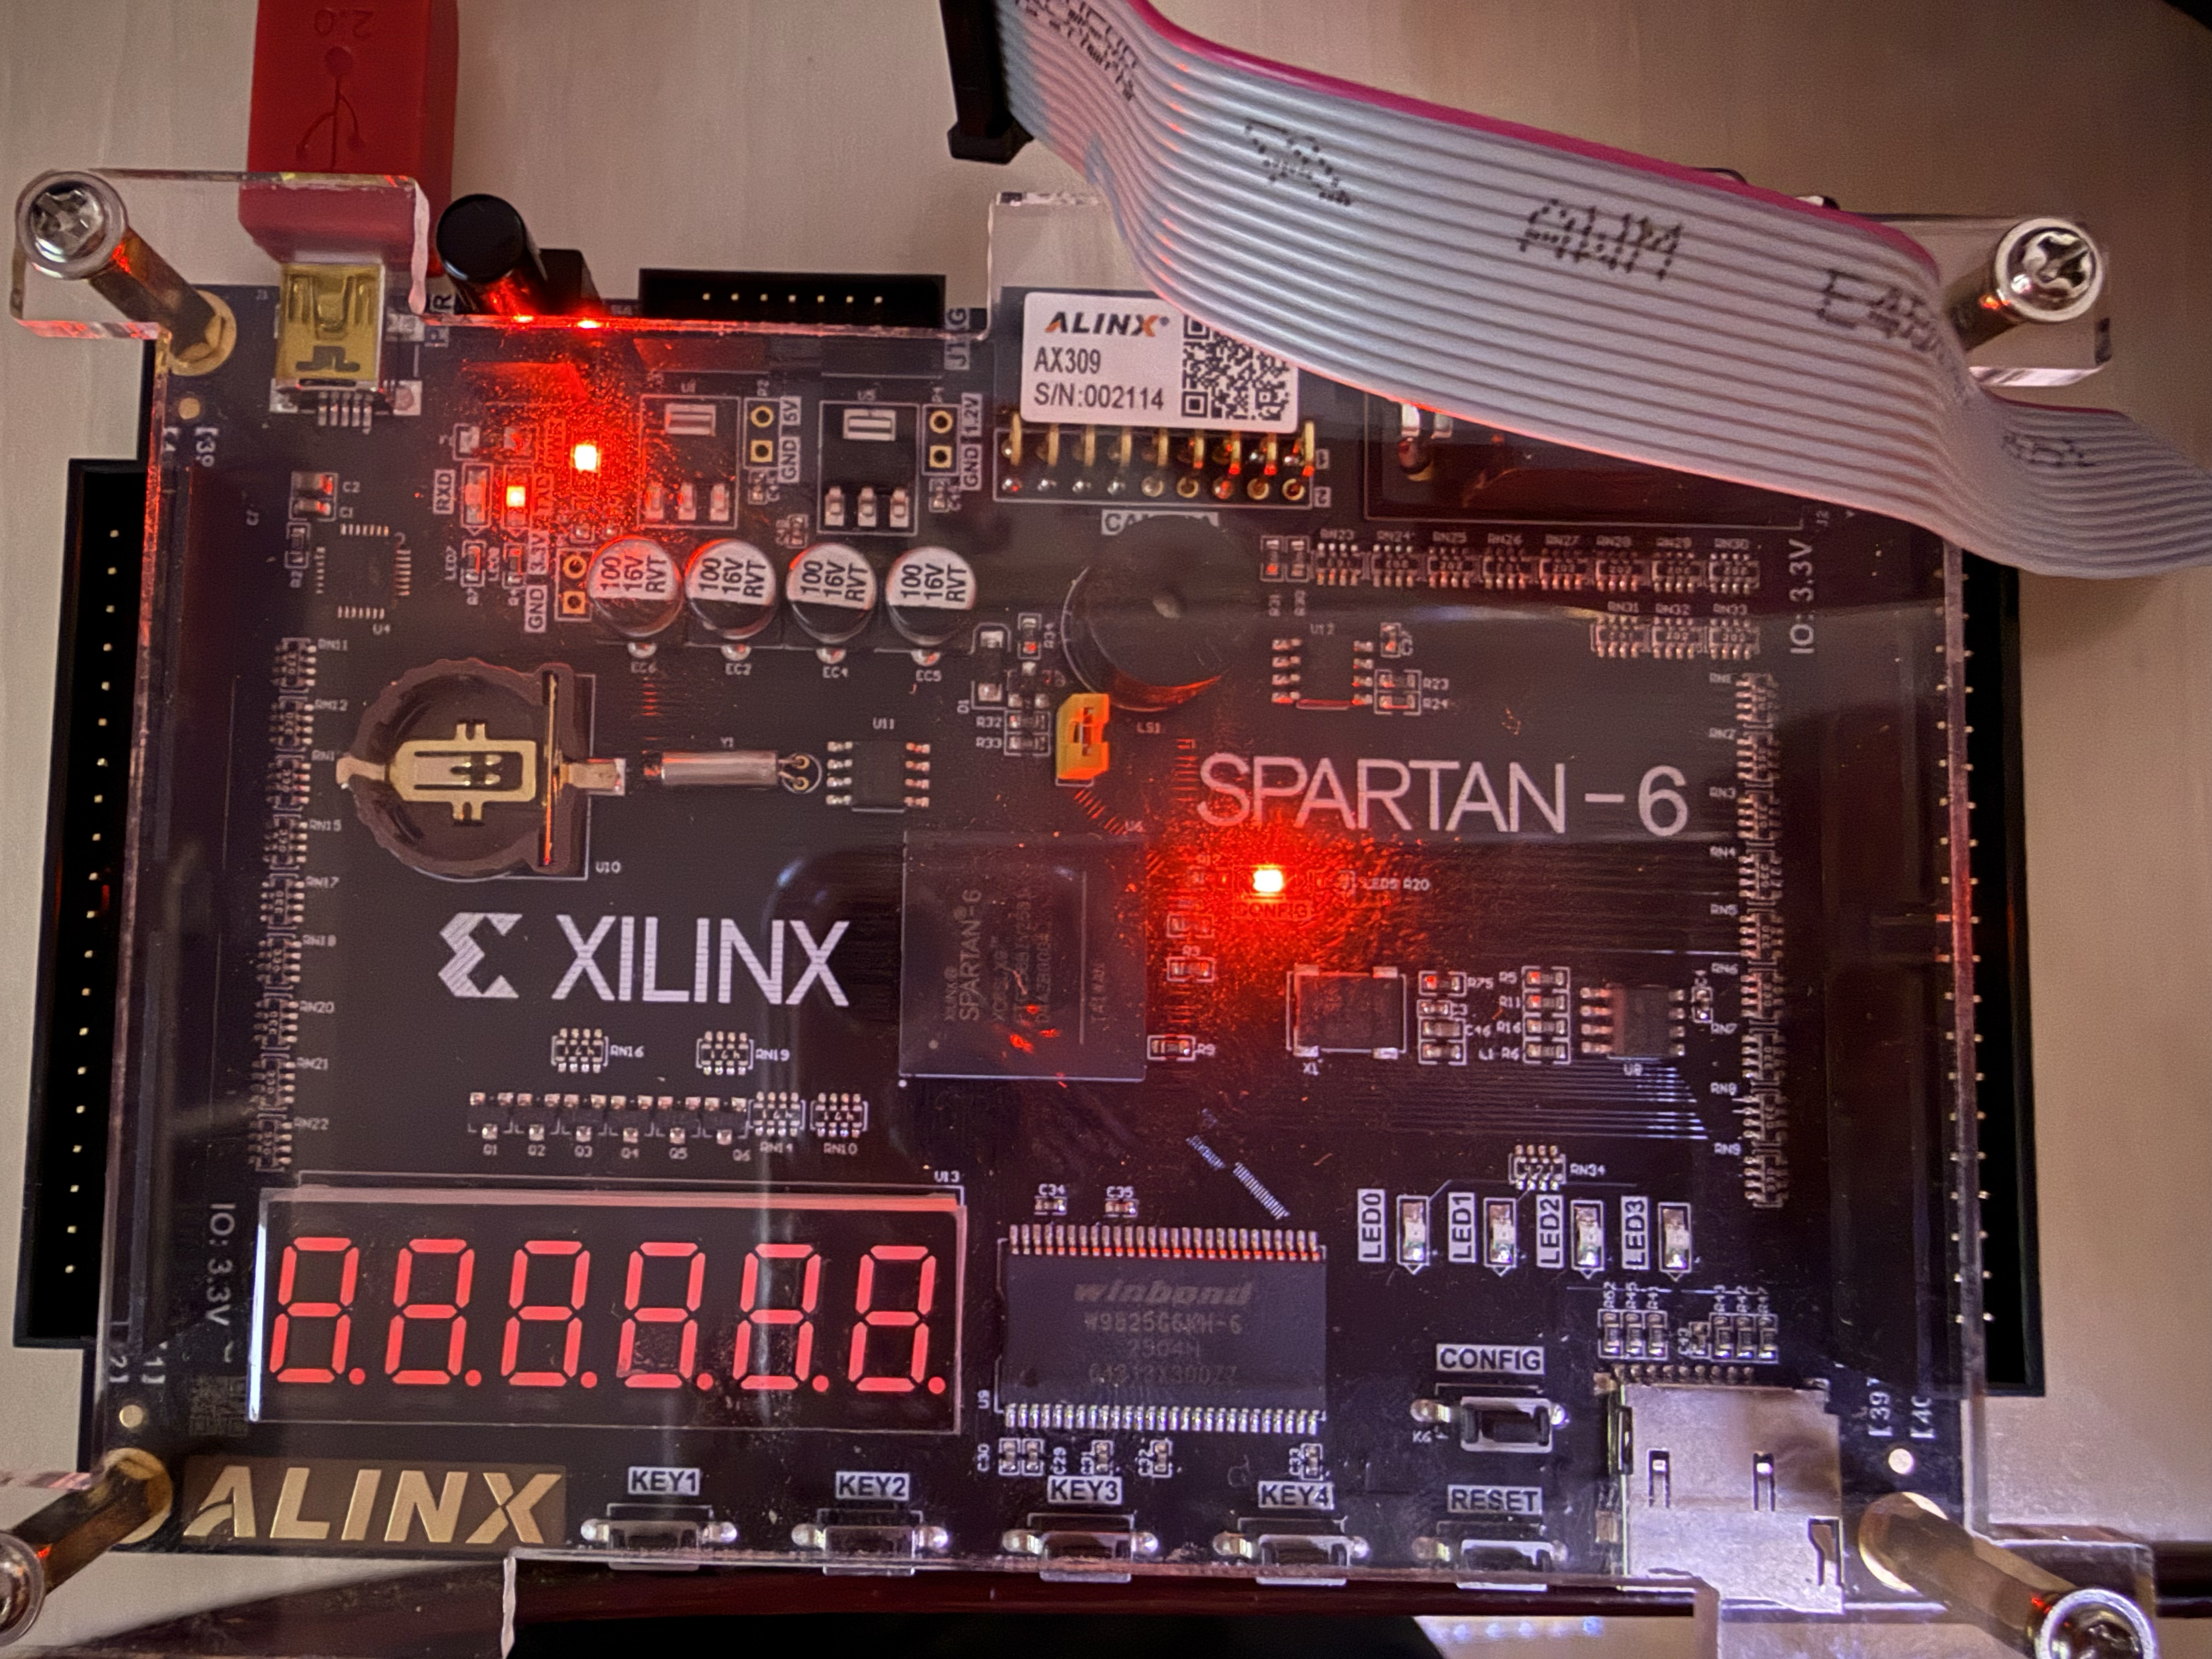
\includegraphics[width=0.8\textwidth]{fpga/fpga_board.png}
    \caption{FPGA 开发板实物连接与测试环境}
\end{figure}

\begin{figure}[H]
    \centering
    \includegraphics[width=0.95\textwidth]{fpga/gtkwave_simulation.png}
    \caption{GHDL + GTKWave 仿真波形:展示了 DDS 查表与正弦波合成}
\end{figure}

\section{附录:项目源代码}

由于篇幅限制,本文档仅列出核心算法的关键实现片段。完整项目(包含 Java Web 后端、前端资源、Python 仿真及 FPGA 工程)已开源。

\textbf{开源仓库地址}:\url{https://github.com/ReragoAliNa/DTMF}

\subsection{Python 核心算法实现 (Goertzel)}
\lstinputlisting[caption={src/core/dsp.py (部分截取)}, language=Python, firstline=1, lastline=45]{../../src/core/dsp.py}

\subsection{FPGA 信号发生器逻辑 (VHDL)}
\lstinputlisting[caption={fpga/dtmf\_generator.vhd (核心逻辑)}, language=VHDL, firstline=40, lastline=108]{../../fpga/dtmf_generator.vhd}





\section{参考文献}
\begin{thebibliography}{9}

\bibitem{ITU-Q23}
ITU-T Recommendation Q.23. (1988). \textit{Technical features of push-button telephone sets}. International Telecommunication Union.

\bibitem{ITU-Q24}
ITU-T Recommendation Q.24. (1988). \textit{Multifrequency push-button signal reception}. International Telecommunication Union.

\bibitem{Goertzel1958}
Goertzel, G. (1958). An Algorithm for the Evaluation of Finite Trigonometric Series. \textit{American Mathematical Monthly}, 65(1), 34-35.

\bibitem{Oppenheim2010}
Oppenheim, A. V., \& Schafer, R. W. (2010). \textit{Discrete-Time Signal Processing} (3rd ed.). Pearson.

\bibitem{Proakis2006}
Proakis, J. G., \& Manolakis, D. G. (2006). \textit{Digital Signal Processing: Principles, Algorithms, and Applications} (4th ed.). Prentice Hall.

\end{thebibliography}


\end{document}
